\documentclass{scrartcl}
\usepackage{fontenc}
\usepackage{booktabs}
\usepackage{caption}
\usepackage{xfrac}
\usepackage{subcaption}

\title{Dispositionspapier zur Studienarbeit\\Generierung künstlicher Trainingsdaten für die Straßenschilderkennung in Fahrzeugen mittels Generative Adversarial Networks}
\author{ Frederik Esau }
\date{01.01.2023}

\begin{document}

\maketitle

\section{Kurzbeschreibung der Arbeit}
In der Automobilindustrie ist ein häufiges Problem, dass zu wenige echte Trainingsdaten für neuronalen Netze existieren. Diese Arbeit bezieht sich dahingehend auf das Thema Straßenschilderkennung. Es soll ein Algorithmus entwickelt werden, der künstliche Bilder von Straßenschildern erzeugt. Als Eingang dient das Piktogramm eines Straßenschildes. Der Algorithmus soll ein möglichst fotorealistisches Bild generieren, auf dem diese Art von Straßenschild zu sehen ist. Zusätzlich sollen verschiedene äußere Einflüsse simuliert werden, die die Straßenschilderkennung in Fahrzeugen erschweren könnten. Dazu zählen etwa Schnee oder ein verwackeltes Bild.

Das Thema bewegt sich im Rahmen des maschinellen Lernens und basiert genauer auf den \emph{Generative Adversarial Networks} (GANs). Also neuronalen Netzen, die künstliche Bilder generieren können, indem sie ein generierendes und ein überprüfendes Netzwerk besitzen. Das Gesamtnetzwerk in dieser Arbeit ist ein sogenanntes \emph{Cycle Consistent Generative Adversarial Network} (CycleGAN). Es besteht aus zwei miteinander gekoppelten GANs.

Zum jetzigen Zeitpunkt liegt ein trainierbares CycleGAN vor, das ausschließlich Bilder für Vortfahrtsschilder generiert. Das Piktogramm wird dafür vor der Generierung zufällig in x-y- und z-Richtung rotiert sowie in seiner Größe skaliert. Die einzelnen neuronalen Netze, aus denen sich das CycleGAN zusammensetzt, sind nicht selber implementiert, sondern verwenden \emph{Unet}-basierte Pix2Pix Modelle [1]. Es wird erwogen, nachträglich auf \emph{Resnet}-basierte Modelle umzusteigen, wie im CycleGAN Paper beschrieben [2].

Ziele für das Netz sind die folgenden: Die Generierung soll auf mindestens 3 Klassen erweitert werden. Außerdem soll das Training so fortschreiten, dass die generierten Bilder klare optische Ähnlichkeiten mit den Bildern des Trainingssatzes besitzen. Eine Metrik, die dies bestimmt, muss noch gefunden werden. Des Weiteren sollen mindestens zwei äußere Einflüsse simuliert werden. Beispielsweise Schnee und ein Verwackeln der Bilder. Die Generierung soll abschließend, wenn genug Zeit zur Implementierung ist, über eine einfache Benutzerschnittstelle gesteuert werden können.

\begin{figure}[h]
	\centering
	\begin{subfigure}[b]{0.13\textwidth}
		\centering
		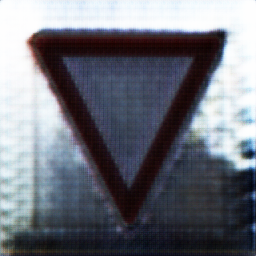
\includegraphics[height=\textwidth]{./images/generierteBilder/0f1c3406-6040-4a1c-8c2f-10b29515b3c3.png}
		\caption{}
		\label{fig:gtrsb-paper-bsp-image-1}
	\end{subfigure}
	\hspace{2em}%
	\begin{subfigure}[b]{0.13\textwidth}
		\centering
		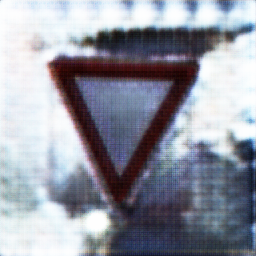
\includegraphics[height=\textwidth]{./images/generierteBilder/02095bc9-6920-425f-9f5b-5e02dbfda540.png}
		\caption{}
		\label{fig:gtrsb-paper-bsp-image-2}
	\end{subfigure}
	\hspace{2em}%
	\begin{subfigure}[b]{0.13\textwidth}
		\centering
		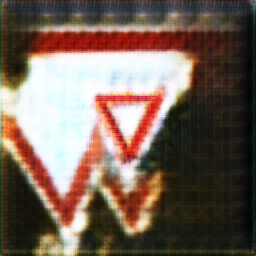
\includegraphics[height=\textwidth]{./images/generierteBilder/c583d04b-f707-4663-a3e3-5deae07c55d7.png}
		\caption{}
		\label{fig:gtrsb-paper-bsp-image-3}
	\end{subfigure}
	\hspace{2em}%
	\begin{subfigure}[b]{0.13\textwidth}
		\centering
		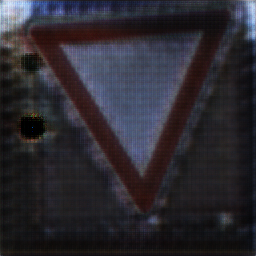
\includegraphics[height=\textwidth]{./images/generierteBilder/e5026964-ec71-4020-9dd4-8324783d4163.png}
		\caption{}
		\label{fig:gtrsb-paper-bsp-image-4}
	\end{subfigure}
	\caption{Momentan generierte Bilder des Netzes}
	\label{fig:gtrsb-paper-bsp-images}
\end{figure}

%\begin{figure}[h]
%	\centering
%	\begin{subfigure}[b]{0.15\textwidth}
%		\centering
%		
\includegraphics[height=\textwidth]{./images/Trainingsfortschritt/64c6a8cd-ac47-46b4-98de-e3d927bf2186.png}
%		\caption{}
%		\label{fig:gtrsb-paper-bsp-image-13245}
%	\end{subfigure}
%	\hspace{2em}%
%	\begin{subfigure}[b]{0.15\textwidth}
%		\centering
%		
\includegraphics[height=\textwidth]{./images/Trainingsfortschritt/dde70277-65bc-40c5-af7c-5c3e2d8fafb2.png}
%		\caption{}
%		\label{fig:gtrsb-paper-bsp-image-3452}
%	\end{subfigure}
%	\hspace{2em}%
%	\begin{subfigure}[b]{0.15\textwidth}
%		\centering
%		
\includegraphics[height=\textwidth]{./images/Trainingsfortschritt/a1844b3d-9001-4dbf-8401-1398e723e460.png}
%		\caption{}
%		\label{fig:gtrsb-paper-bsp-image-3453}
%	\end{subfigure}
%	\hspace{2em}%
%	\begin{subfigure}[b]{0.15\textwidth}
%		\centering
%		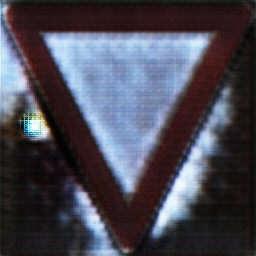
\includegraphics[height=\textwidth]{./images/Trainingsfortschritt/2141ab32-b60d-4897-ba0c-b7fdbada919b.png}
%		\caption{}
%		\label{fig:gtrsb-paper-bsp-image-43456}
%	\end{subfigure}
%	\caption{Trainingsfortschritt (Epochen 1-200)}
%	\label{fig:gtrsb-paper-bsp-images345}
%\end{figure}


\section{Gliederung und Zeitplan}
Die wesentlichen Arbeitschritte sind: Einarbeitung in das Thema, Konzeption und Implementierung der Bildgenerierung, Erweiterung um die Generierung äußerer Einflüsse, Evaluation. Die Einarbeitung findet dabei nicht vollständig voher statt, sondern während der Umsetzung.

Die gesamte Arbeit soll bis Anfang Mai fertig sein. Die Zeit von Mai bis Juni dient als Puffer.

\begin{description}
	\item[1 Einleitung] Problemstellung, Ziel der Arbeit, Vorgehensweise
	\item[2 Stand der Technik] Straßenschilderkennung, künstliche neuronale Netze, Bildgenerierung, Vorherige Arbeiten, Machine Learning Frameworks
	\item[3 Konzeption des Netzwerks] Datensatz, Framework, Architektur, Datenaufbereitung, Training
	\item[4 Implementierung und Training] Hyperparameter, Hinzufügen äußerer Einflüsse
	\item[5 Evaluation] Metrik zur Erfassung der Performanz, Vergleich von Unet und Resnet
	\item[6 Zusammenfassung]
	
\end{description}

\section{Grundlegende Literatur}
Zwei Paper wurden gefunden, die grundsätzlich das gleiche Thema behandeln [3][4]. Eines der Paper verwendet den gleichen Datensatz [3]. Die Erkenntnisse daraus verwendet diese Arbeit als Basis. Keine der gefundenen Literatur bezieht sich explizit auf die Simulation äußerer Einflüsse, die die Straßenschilderkennung erschweren könnten. Dies stellt hier den neuen Anteil dar. In Paper [3] wird dies als zukünftiges Ziel definiert.
\newline\newline [1] arXiv:1611.07004v3 [2] 10.48550/ARXIV.1703.10593 [3] 10.1109/IVS.2019.8814090 [4] 10.1007/s00521-021-05982-z

\end{document}
